\section{Wm4::Intr\-Segment3Triangle3$<$ Real $>$ Class Template Reference}
\label{classWm4_1_1IntrSegment3Triangle3}\index{Wm4::IntrSegment3Triangle3@{Wm4::IntrSegment3Triangle3}}
{\tt \#include $<$Wm4Intr\-Segment3Triangle3.h$>$}

Collaboration diagram for Wm4::Intr\-Segment3Triangle3$<$ Real $>$:\begin{figure}[H]
\begin{center}
\leavevmode
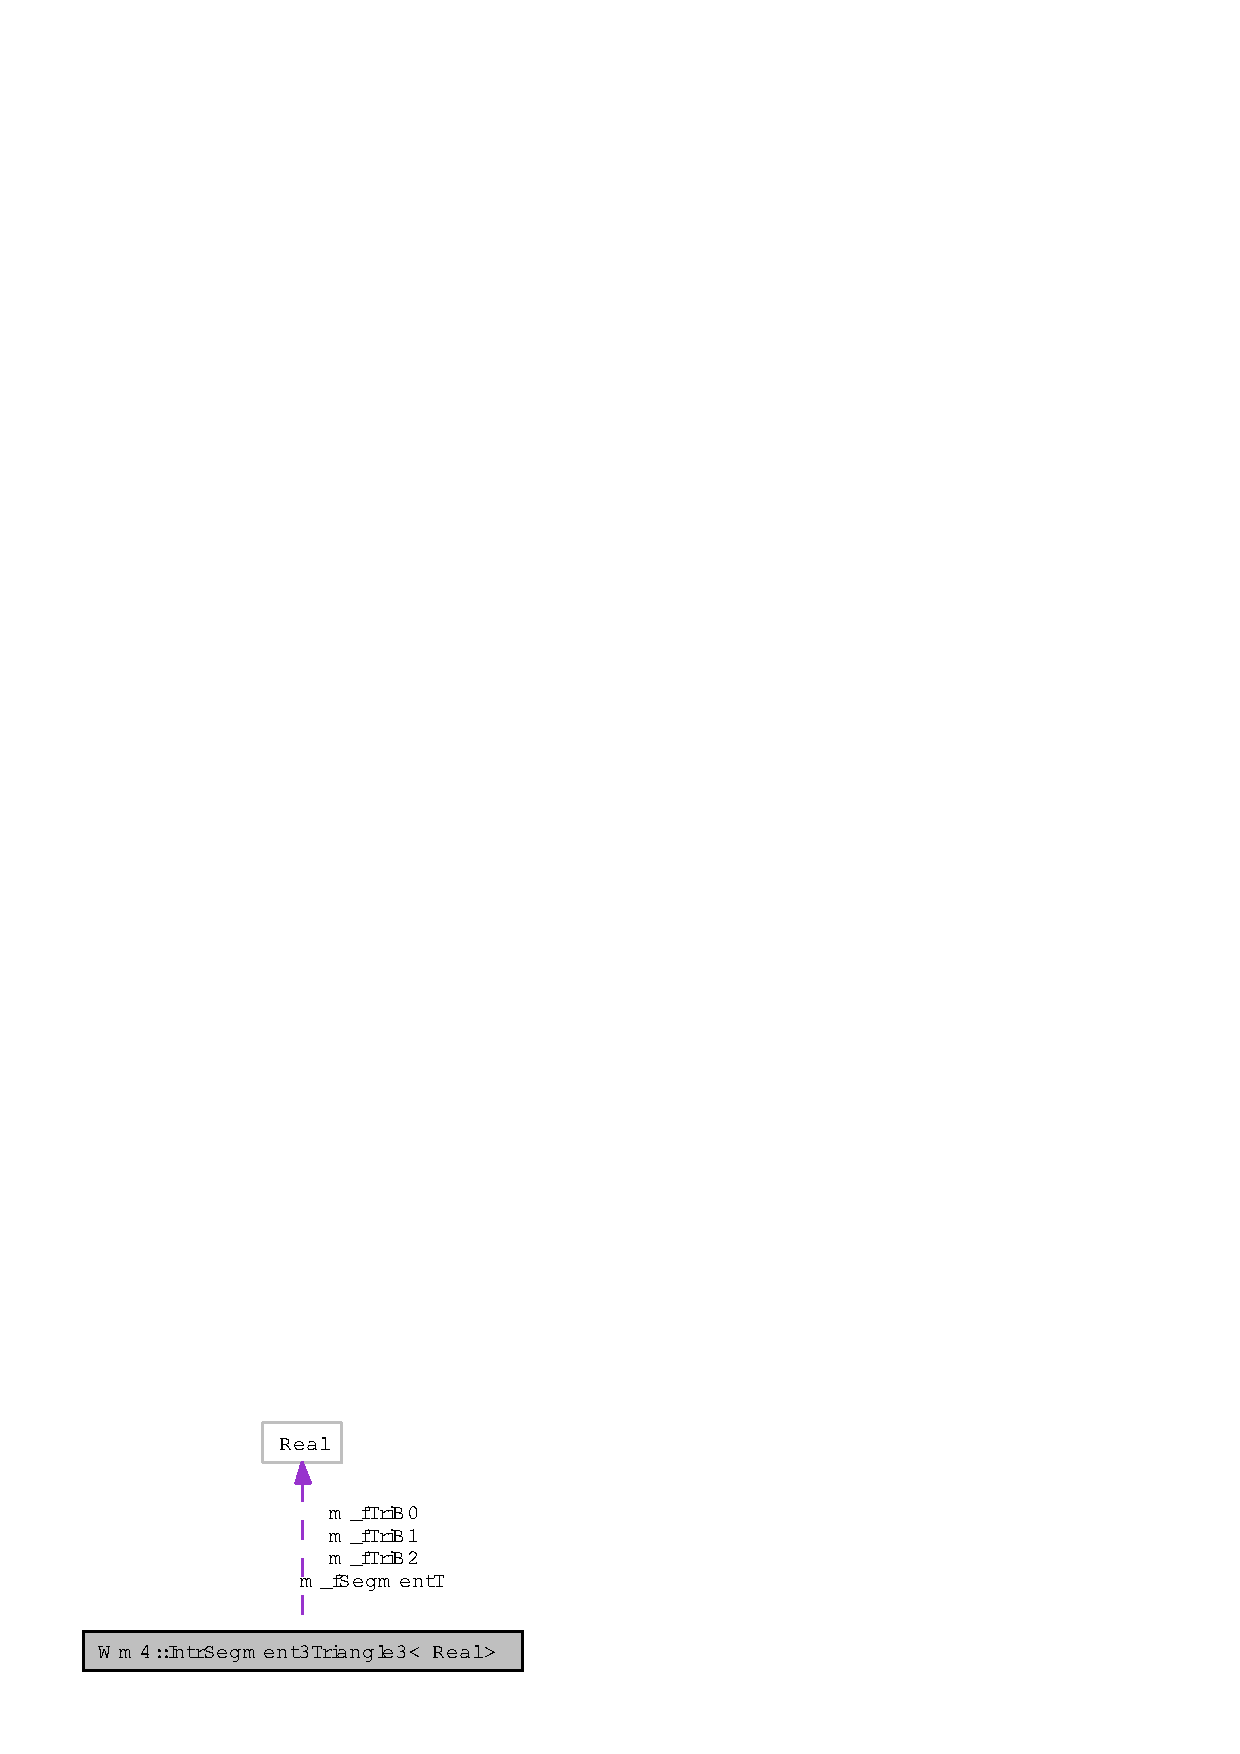
\includegraphics[width=127pt]{classWm4_1_1IntrSegment3Triangle3__coll__graph}
\end{center}
\end{figure}
\subsection*{Public Member Functions}
\begin{CompactItemize}
\item 
{\bf Intr\-Segment3Triangle3} (const Segment3$<$ Real $>$ \&rk\-Segment, const Triangle3$<$ Real $>$ \&rk\-Triangle)
\item 
const Segment3$<$ Real $>$ \& {\bf Get\-Segment} () const
\item 
const Triangle3$<$ Real $>$ \& {\bf Get\-Triangle} () const
\item 
virtual bool {\bf Test} ()
\item 
virtual bool {\bf Find} ()
\item 
Real {\bf Get\-Segment\-T} () const
\item 
Real {\bf Get\-Tri\-B0} () const
\item 
Real {\bf Get\-Tri\-B1} () const
\item 
Real {\bf Get\-Tri\-B2} () const
\item 
virtual bool {\bf Test} (Real f\-TMax, const {\bf Vector3}$<$ Real $>$ \&rk\-Velocity0, const {\bf Vector3}$<$ Real $>$ \&rk\-Velocity1)
\item 
virtual bool {\bf Find} (Real f\-TMax, const {\bf Vector3}$<$ Real $>$ \&rk\-Velocity0, const {\bf Vector3}$<$ Real $>$ \&rk\-Velocity1)
\item 
int {\bf Get\-Quantity} () const
\item 
const {\bf Vector3}$<$ Real $>$ \& {\bf Get\-Point} (int i) const
\end{CompactItemize}
\subsubsection*{template$<$class Real$>$ class Wm4::Intr\-Segment3Triangle3$<$ Real $>$}



\subsection{Constructor \& Destructor Documentation}
\index{Wm4::IntrSegment3Triangle3@{Wm4::Intr\-Segment3Triangle3}!IntrSegment3Triangle3@{IntrSegment3Triangle3}}
\index{IntrSegment3Triangle3@{IntrSegment3Triangle3}!Wm4::IntrSegment3Triangle3@{Wm4::Intr\-Segment3Triangle3}}
\subsubsection{\setlength{\rightskip}{0pt plus 5cm}template$<$class Real$>$ {\bf Wm4::Intr\-Segment3Triangle3}$<$ Real $>$::{\bf Intr\-Segment3Triangle3} (const Segment3$<$ Real $>$ \& {\em rk\-Segment}, const Triangle3$<$ Real $>$ \& {\em rk\-Triangle})}\label{classWm4_1_1IntrSegment3Triangle3_ae90a2770821bb24ea659d635c919176}




\subsection{Member Function Documentation}
\index{Wm4::IntrSegment3Triangle3@{Wm4::Intr\-Segment3Triangle3}!GetSegment@{GetSegment}}
\index{GetSegment@{GetSegment}!Wm4::IntrSegment3Triangle3@{Wm4::Intr\-Segment3Triangle3}}
\subsubsection{\setlength{\rightskip}{0pt plus 5cm}template$<$class Real$>$ const Segment3$<$ Real $>$ \& {\bf Wm4::Intr\-Segment3Triangle3}$<$ Real $>$::Get\-Segment () const}\label{classWm4_1_1IntrSegment3Triangle3_b32213d1a8556d80f3da862d80b78408}


\index{Wm4::IntrSegment3Triangle3@{Wm4::Intr\-Segment3Triangle3}!GetTriangle@{GetTriangle}}
\index{GetTriangle@{GetTriangle}!Wm4::IntrSegment3Triangle3@{Wm4::Intr\-Segment3Triangle3}}
\subsubsection{\setlength{\rightskip}{0pt plus 5cm}template$<$class Real$>$ const Triangle3$<$ Real $>$ \& {\bf Wm4::Intr\-Segment3Triangle3}$<$ Real $>$::Get\-Triangle () const}\label{classWm4_1_1IntrSegment3Triangle3_5cc684c2193aa0741761d32aef70e702}


\index{Wm4::IntrSegment3Triangle3@{Wm4::Intr\-Segment3Triangle3}!Test@{Test}}
\index{Test@{Test}!Wm4::IntrSegment3Triangle3@{Wm4::Intr\-Segment3Triangle3}}
\subsubsection{\setlength{\rightskip}{0pt plus 5cm}template$<$class Real$>$ bool {\bf Wm4::Intr\-Segment3Triangle3}$<$ Real $>$::Test ()\hspace{0.3cm}{\tt  [virtual]}}\label{classWm4_1_1IntrSegment3Triangle3_d4805ab9e7f40f421b7271ea057e2fcb}


\index{Wm4::IntrSegment3Triangle3@{Wm4::Intr\-Segment3Triangle3}!Find@{Find}}
\index{Find@{Find}!Wm4::IntrSegment3Triangle3@{Wm4::Intr\-Segment3Triangle3}}
\subsubsection{\setlength{\rightskip}{0pt plus 5cm}template$<$class Real$>$ bool {\bf Wm4::Intr\-Segment3Triangle3}$<$ Real $>$::Find ()\hspace{0.3cm}{\tt  [virtual]}}\label{classWm4_1_1IntrSegment3Triangle3_cbce364d2d648f6dc0628f28cf88b8b2}


\index{Wm4::IntrSegment3Triangle3@{Wm4::Intr\-Segment3Triangle3}!GetSegmentT@{GetSegmentT}}
\index{GetSegmentT@{GetSegmentT}!Wm4::IntrSegment3Triangle3@{Wm4::Intr\-Segment3Triangle3}}
\subsubsection{\setlength{\rightskip}{0pt plus 5cm}template$<$class Real$>$ Real {\bf Wm4::Intr\-Segment3Triangle3}$<$ Real $>$::Get\-Segment\-T () const}\label{classWm4_1_1IntrSegment3Triangle3_3c4873255c7a4bdf3d71f22c3d557118}


\index{Wm4::IntrSegment3Triangle3@{Wm4::Intr\-Segment3Triangle3}!GetTriB0@{GetTriB0}}
\index{GetTriB0@{GetTriB0}!Wm4::IntrSegment3Triangle3@{Wm4::Intr\-Segment3Triangle3}}
\subsubsection{\setlength{\rightskip}{0pt plus 5cm}template$<$class Real$>$ Real {\bf Wm4::Intr\-Segment3Triangle3}$<$ Real $>$::Get\-Tri\-B0 () const}\label{classWm4_1_1IntrSegment3Triangle3_e0552d572714bf9d22d2cd74c4362f9b}


\index{Wm4::IntrSegment3Triangle3@{Wm4::Intr\-Segment3Triangle3}!GetTriB1@{GetTriB1}}
\index{GetTriB1@{GetTriB1}!Wm4::IntrSegment3Triangle3@{Wm4::Intr\-Segment3Triangle3}}
\subsubsection{\setlength{\rightskip}{0pt plus 5cm}template$<$class Real$>$ Real {\bf Wm4::Intr\-Segment3Triangle3}$<$ Real $>$::Get\-Tri\-B1 () const}\label{classWm4_1_1IntrSegment3Triangle3_ffc0a298a3a668c7052fb9b29f70d754}


\index{Wm4::IntrSegment3Triangle3@{Wm4::Intr\-Segment3Triangle3}!GetTriB2@{GetTriB2}}
\index{GetTriB2@{GetTriB2}!Wm4::IntrSegment3Triangle3@{Wm4::Intr\-Segment3Triangle3}}
\subsubsection{\setlength{\rightskip}{0pt plus 5cm}template$<$class Real$>$ Real {\bf Wm4::Intr\-Segment3Triangle3}$<$ Real $>$::Get\-Tri\-B2 () const}\label{classWm4_1_1IntrSegment3Triangle3_e94f5488046b1331cf02f6a78618ffa4}


\index{Wm4::IntrSegment3Triangle3@{Wm4::Intr\-Segment3Triangle3}!Test@{Test}}
\index{Test@{Test}!Wm4::IntrSegment3Triangle3@{Wm4::Intr\-Segment3Triangle3}}
\subsubsection{\setlength{\rightskip}{0pt plus 5cm}template$<$class Real$>$ bool {\bf Wm4::Intr\-Segment3Triangle3}$<$ Real $>$::Test (Real {\em f\-TMax}, const {\bf Vector3}$<$ Real $>$ \& {\em rk\-Velocity0}, const {\bf Vector3}$<$ Real $>$ \& {\em rk\-Velocity1})\hspace{0.3cm}{\tt  [virtual]}}\label{classWm4_1_1IntrSegment3Triangle3_ec56edb6e1a5e4a3eab61b90d21d3180}


\index{Wm4::IntrSegment3Triangle3@{Wm4::Intr\-Segment3Triangle3}!Find@{Find}}
\index{Find@{Find}!Wm4::IntrSegment3Triangle3@{Wm4::Intr\-Segment3Triangle3}}
\subsubsection{\setlength{\rightskip}{0pt plus 5cm}template$<$class Real$>$ bool {\bf Wm4::Intr\-Segment3Triangle3}$<$ Real $>$::Find (Real {\em f\-TMax}, const {\bf Vector3}$<$ Real $>$ \& {\em rk\-Velocity0}, const {\bf Vector3}$<$ Real $>$ \& {\em rk\-Velocity1})\hspace{0.3cm}{\tt  [virtual]}}\label{classWm4_1_1IntrSegment3Triangle3_14b6137039fc467396424e8b5e6716aa}


\index{Wm4::IntrSegment3Triangle3@{Wm4::Intr\-Segment3Triangle3}!GetQuantity@{GetQuantity}}
\index{GetQuantity@{GetQuantity}!Wm4::IntrSegment3Triangle3@{Wm4::Intr\-Segment3Triangle3}}
\subsubsection{\setlength{\rightskip}{0pt plus 5cm}template$<$class Real$>$ int {\bf Wm4::Intr\-Segment3Triangle3}$<$ Real $>$::Get\-Quantity () const}\label{classWm4_1_1IntrSegment3Triangle3_1c9ecd76e19183d907ca8d57e864ed7b}


\index{Wm4::IntrSegment3Triangle3@{Wm4::Intr\-Segment3Triangle3}!GetPoint@{GetPoint}}
\index{GetPoint@{GetPoint}!Wm4::IntrSegment3Triangle3@{Wm4::Intr\-Segment3Triangle3}}
\subsubsection{\setlength{\rightskip}{0pt plus 5cm}template$<$class Real$>$ const {\bf Vector3}$<$ Real $>$ \& {\bf Wm4::Intr\-Segment3Triangle3}$<$ Real $>$::Get\-Point (int {\em i}) const}\label{classWm4_1_1IntrSegment3Triangle3_04684d5627edf7335bac7730cf4767a7}




The documentation for this class was generated from the following files:\begin{CompactItemize}
\item 
{\bf Wm4Intr\-Segment3Triangle3.h}\item 
{\bf Wm4Intr\-Segment3Triangle3.cpp}\end{CompactItemize}
